\chapter*{5 - Sumador BCD}
\section{Objetivo}
  Un sumador BCD posee una funci\'on bastante autoexplicativa, esta es la de tomar 2 valores en expresi\'on binaria y presentar la suma de esta en un formato BCD.
  \section{Implementaci\'ion}
  A la hora de desarrollar el programa se han tenido en cuenta los conceptos de modularizaci\'on y reutilizaci\'on de codigo por lo que este ha comprendido distintas etapas con sus propias funcionalidades. Por lo tanto la implementaci\'on final del codigo ha comprendido distitas estapas las cuales se aboradaran a continuaci\'on.
  \subsection{Adder de 1bit}
  El primer circuito l\'ogico necesario para todas las siguientes implementaciones fue sumador de 1 bit, este tiene la funci\'on de realizar la suma de 2 valores de un bit arrojando como parametros de salida tanto el bit resultante como el bit \emph{carry} generado por estos. este circuito se logra realizando una funci\'on AND a los parametros de entrada, llamese estos \emph{A} y \emph{B}, obteniendo de ese modo el bit de salida \emph{Y} y paralelamente realizando una funcion XOR a los mismos y definiendo de ese modo el valor carry de salida. Este circuito se puede ver representado en el siguiente diagrama:
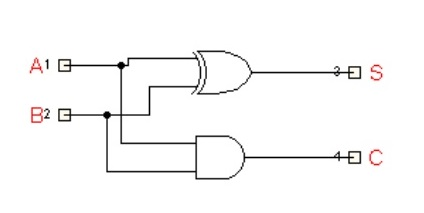
\includegraphics[width=\textwidth]{Ejercicios/adder.jpg}
\subsection{Full-Adder de 1bit}
 Una vez obtenido el Adder se implementa este para lograr el Full-Adder de un bit el cual cumple las mismas funciones basicas con la salvedad que este es capaz de recibir ademas un bit carry como parametro de entrada. Las funciones que cumple el Adder de un bit en el funcionamiento del Full Adder son las siguientes, en primer lugar se tratan los bit de entrara \emph{A} y \emph{B}, estos son aplicados al Adder de ese modo obteniendo un bit de carry que llamaremos \emph{Co1} y una salida \emph{Y1}, lo siguiente sera realizar un Adder con los valores Y1 y el carry de entrada \emph{Cin}, una vez en este punto ya tendremos el bit de salida deasado junto con un segundo bit carry de salida, llamese \emph{Co2}, por lo que resta definir cual sera el bit de carry a la salida del circuito. Este ultimo se obtiene realizando una función OR a los 2 bits carry \emph{Co1} y \emph{Co2}. A continuación se muestra el diagrama del Full-Adder de 1 bit:
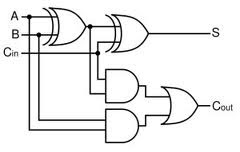
\includegraphics[width=\textwidth]{Ejercicios/full adder.jpg}
\subsection{Full-Adder de 4 bits}
  Contando ya con el Full Adder de 1 bit se escala el funcionamiento de este para lograr realizar la función de suma para valores binarios de 4 bits. Para ello el procedimiento que se realiza es el de tomar de a pares los bits que componen los nibbles con los que se trabaja comenzando por los menos significativos, estos son tratados con el Full Adder (siendo el bit carry de entrada 0) y de aqui se obtiene el bit menos significativo del nibble de salida, por otro lado el bit carry que se obtinene sera el mismo ingresado como el de entrada al Full Adder al que se ingresaran los siguientes bits de los nibbles de entrada. Asi se obtendran los bits de salida yendo del menos significativo al mas significativo y, a su vez, el bit carry de salida producto del ultimo Full Adder de 1 bit implementado sera el que determine si se produjo carry al finalizar la suma.
\\
\subsection{Diseño del Sumador BCD}
  Una vez contando con todas estas herramientas nos disponemos a desarrollar el sumador BCD, para esto el procedimiento a seguir es el siguiente. El suamdor recibira como parametros de entrada 2 nibbles que se llamaran \emph{A} y \emph{B} estos seran ingresados a un bloque Full-Adder de 4 bits, el cual como se sabe devolvera el nibble de salida junto con el bit carry generado, con estos datos se veran si se cumplen alguna de las siguientes condiciones: por un lado si el nibble de salida comprende un numero decimal mayor a 9, o si se ha producido carry en la suma, esto determinara el valor de una señal que actuara como selector de un dispositivo MUX, el cual dependiendo del estado del selector arrojara a la salida un valor decimal de 6, el cual sera el factor de corrección que convierta el valor en expresión binaria a BCD,  o un valor nulo. Por último se tomara el nibble de salida del bloque Adder anterior y el valor a la salida del MUX y se haran pasar estos por un nuevo bloque Full-Adder de 4 bits el cual devolvera un nuevo nibble de salida y el carry de la suma. El criterio que se siguio fue el de devolver el nibble menos significtivo de la suma y un bit carry que indique si el mas significativo comprende un 1 o 0, debido a que la suma de 2 números dara un valor por debajo de 20. Se aclara ademas que la operación se suma de hizo robusta de tal menera que también informara si los parametros de entrada no son validos